%DO NOT MESS AROUND WITH THE CODE ON THIS PAGE UNLESS YOU %REALLY KNOW WHAT YOU ARE DOING
\chapter{Experimental research} \label{Experimental research}

\section{ Comparision of the results of different empirical formulae } \label{Comparision of the results of different empirical formulae}
\noindent By using the empirical formulae of Thorp, Schulkin and Marsh, Francois and Garrison's models to calculate the attenuation coefficient , the graph of attenuation coefficient versus frequency is plotted and compared.

\begin{figure}[H]
\centering
{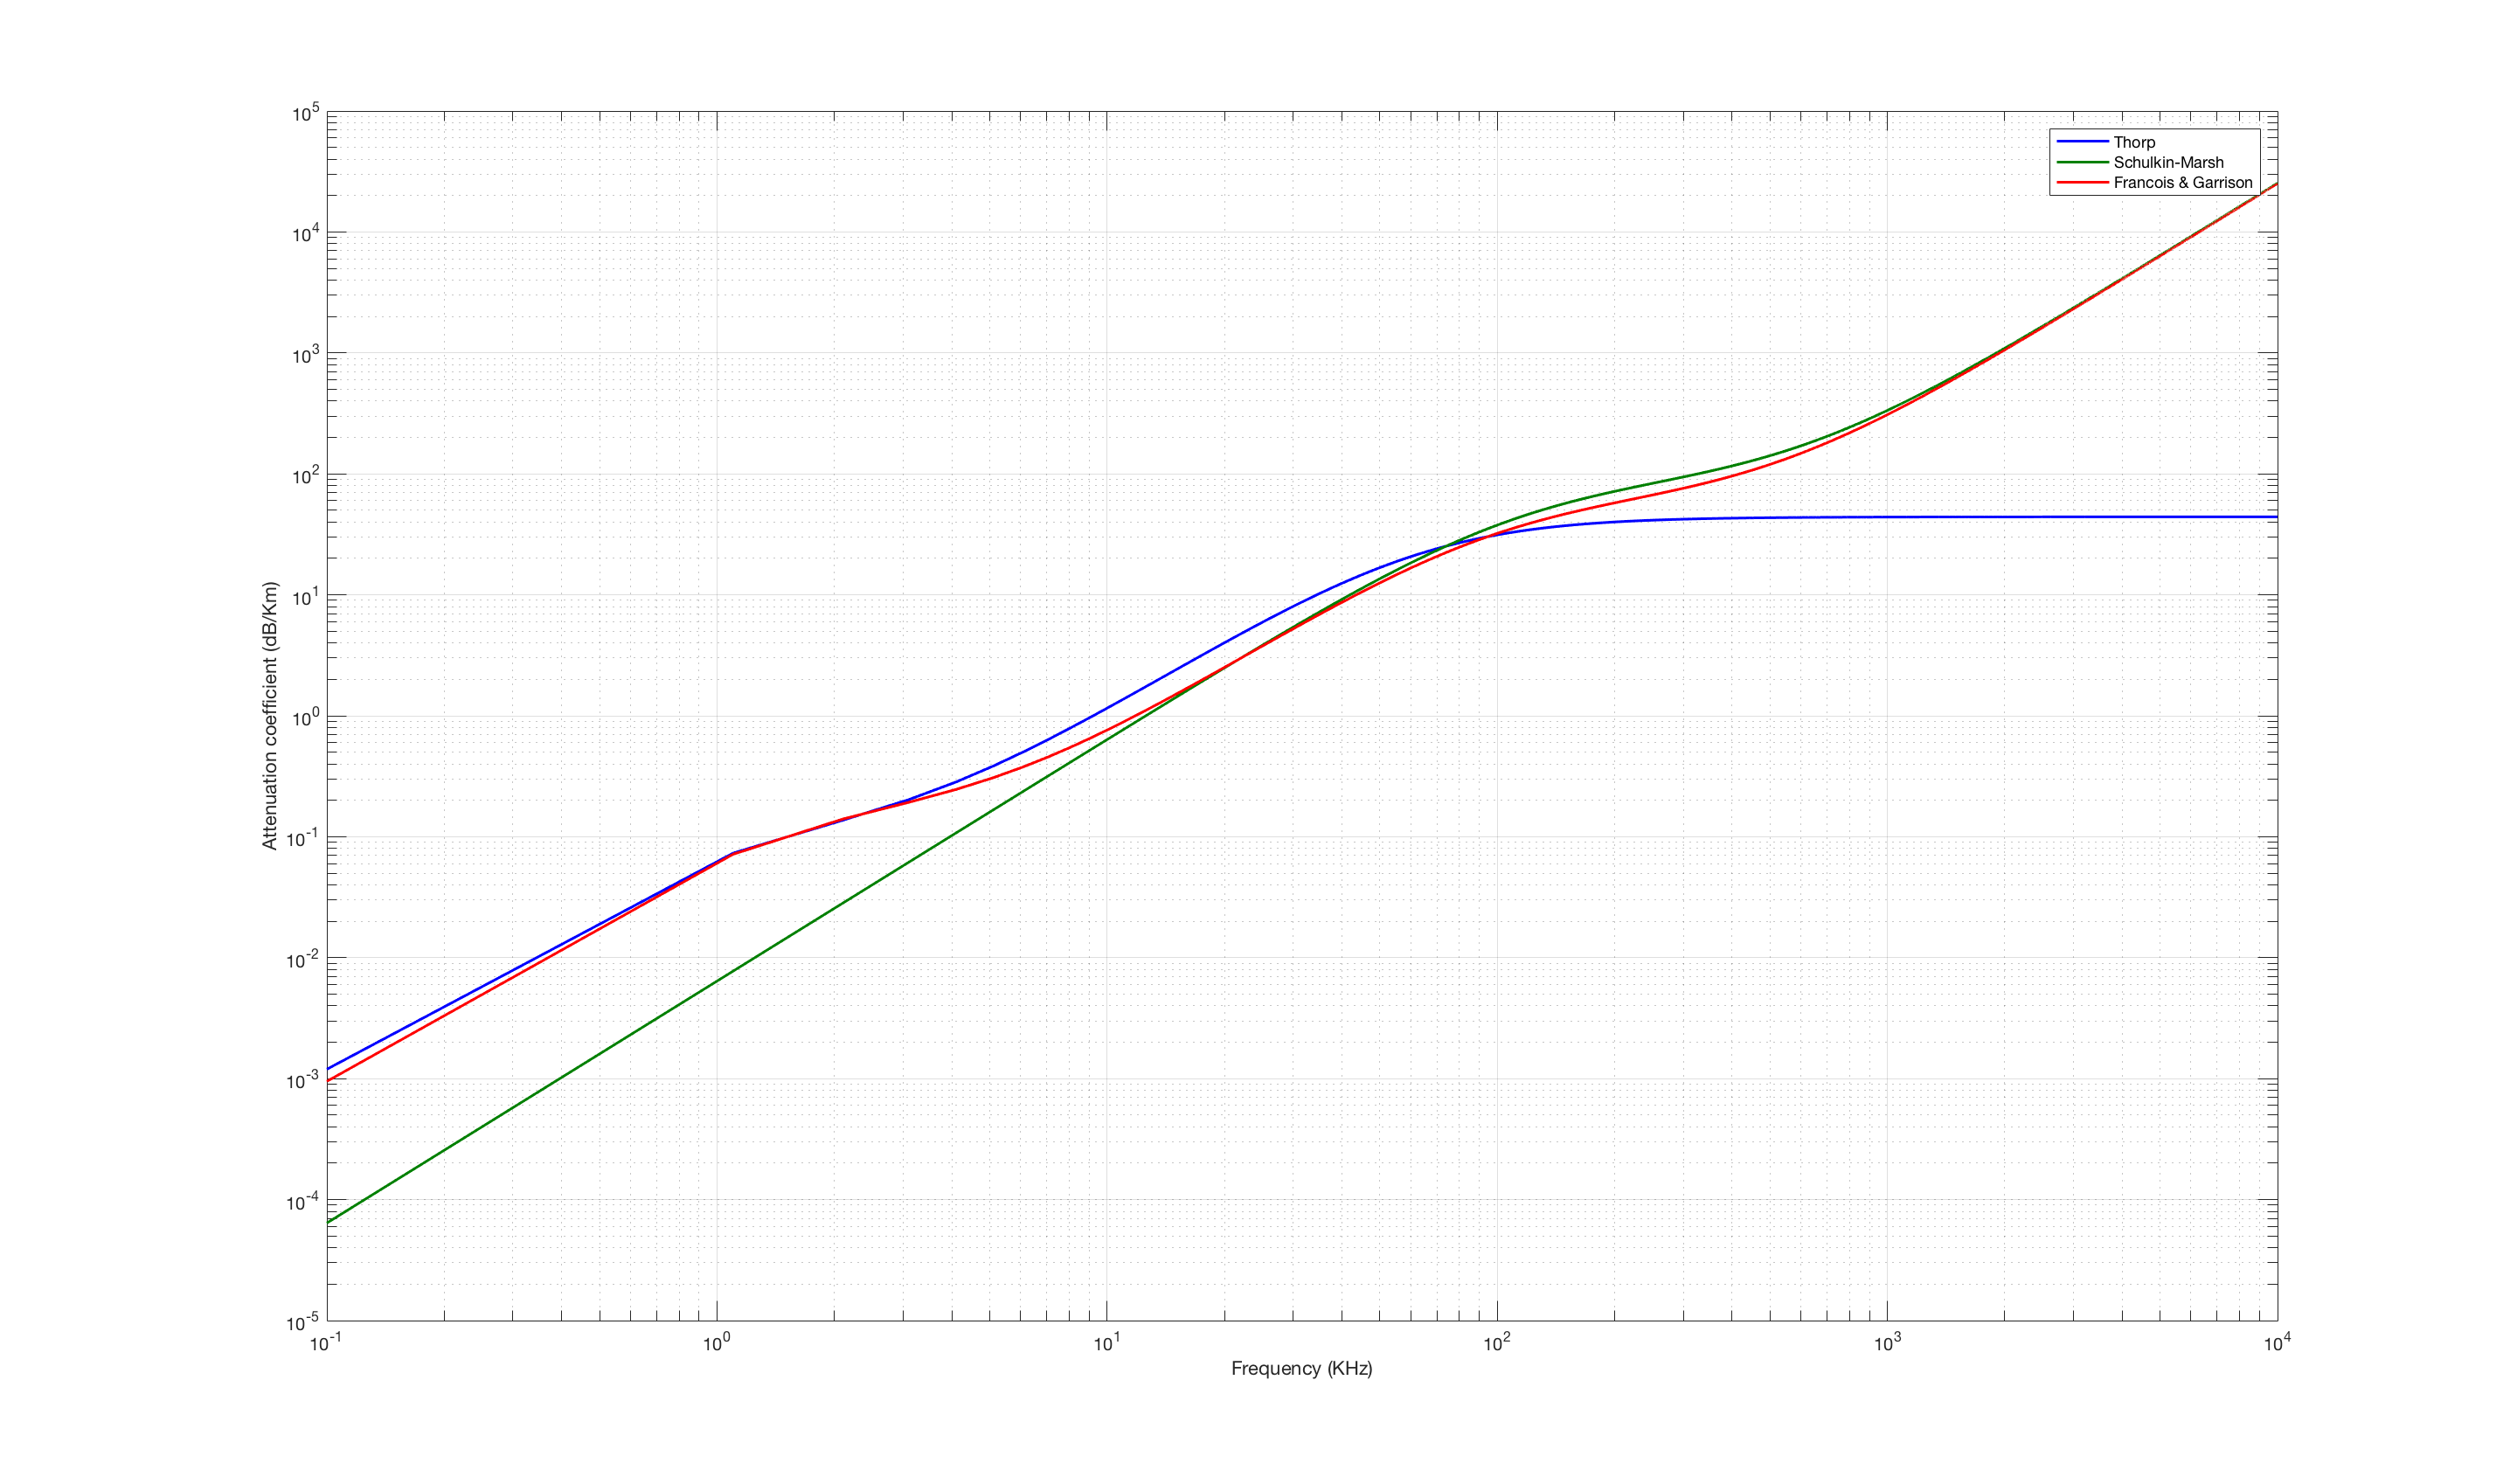
\includegraphics[scale=0.15]{ucp2_1.png}}
\caption{Comparision of different empirical formulae}
\end{figure}

\section{Dependence of attenuation coefficient on different parameters for Francois and Garrison's model} \label{Dependence of attenuation coefficient on different parameters for Francois and Garrison's model} 
\subsection{Dependence on frequency} \label{Dependence on frequency} 
\noindent A graph of frequency versus attenuation coefficient is plotted for a depth of 50m by keeping temperature and salinity constant and varying frequency. This graph is done in-order to check how each factor contributes to the attenuation coefficient.
\begin{figure}[H]
\centering
{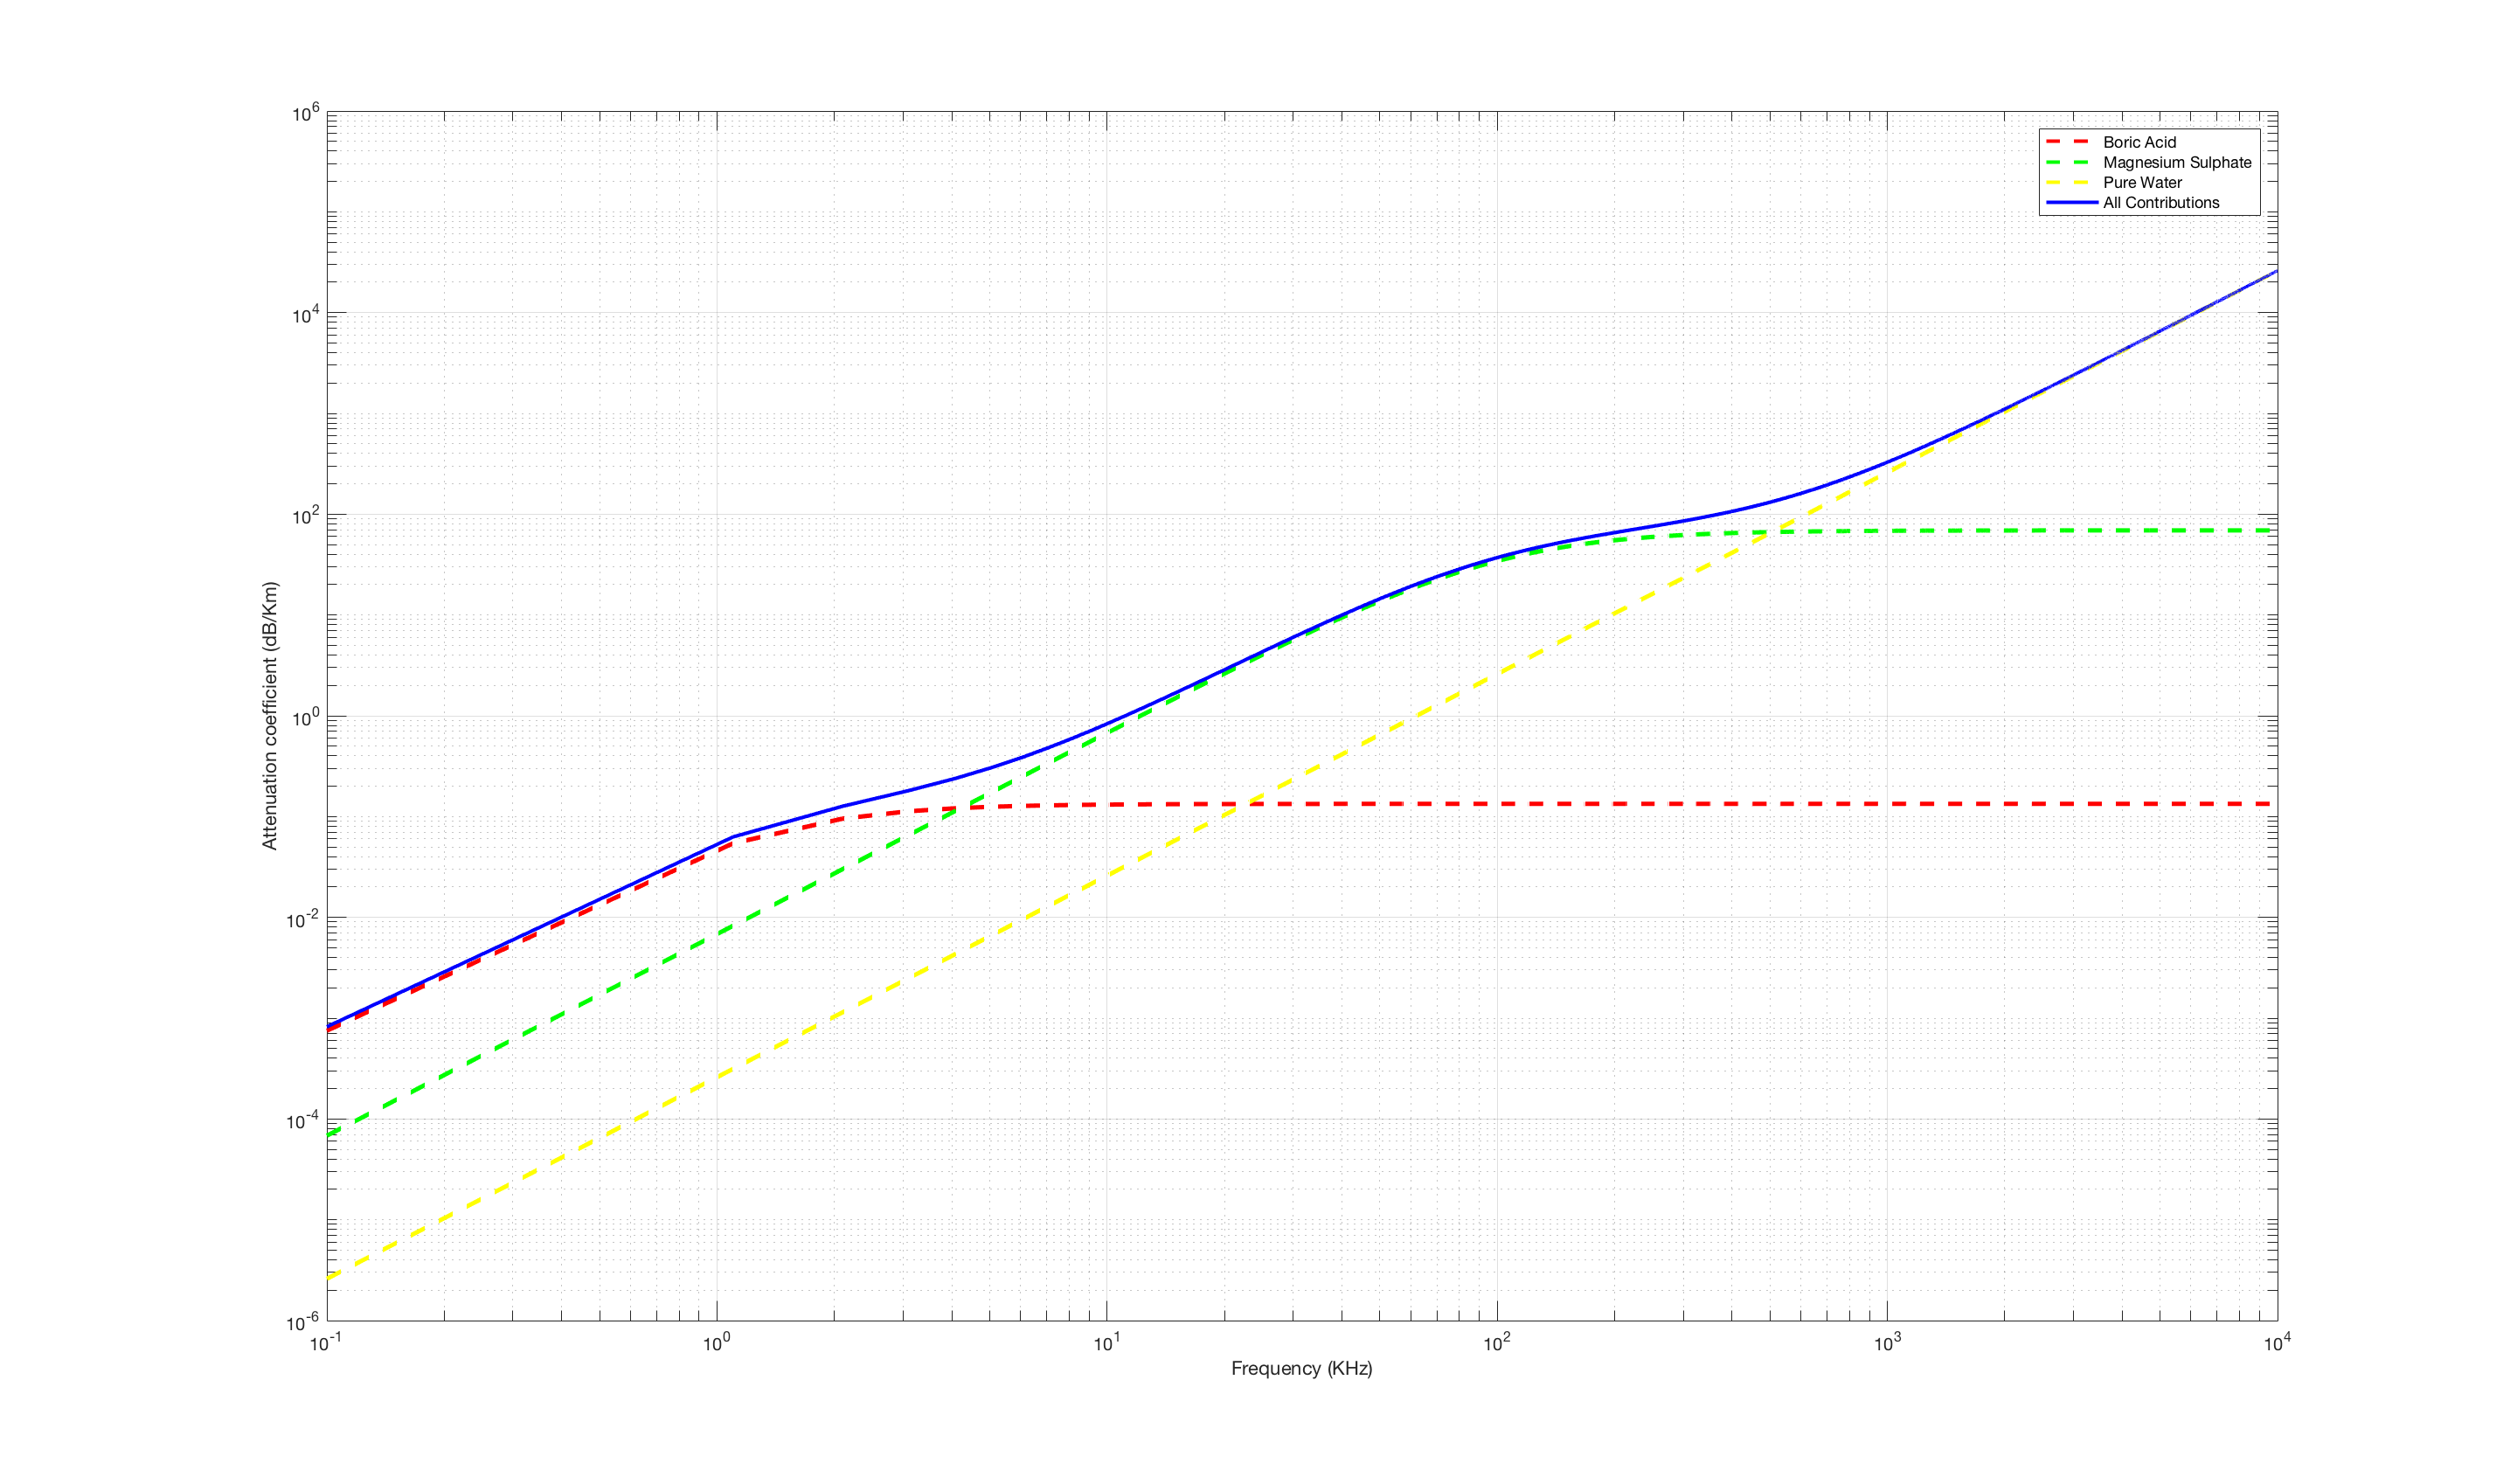
\includegraphics[scale=0.15]{ucp2_2.png}}
\caption{Dependency on frequency}
\end{figure}

\subsection{Dependence on salinity} \label{Dependence on salinity} 

\begin{figure}[H]
\centering
{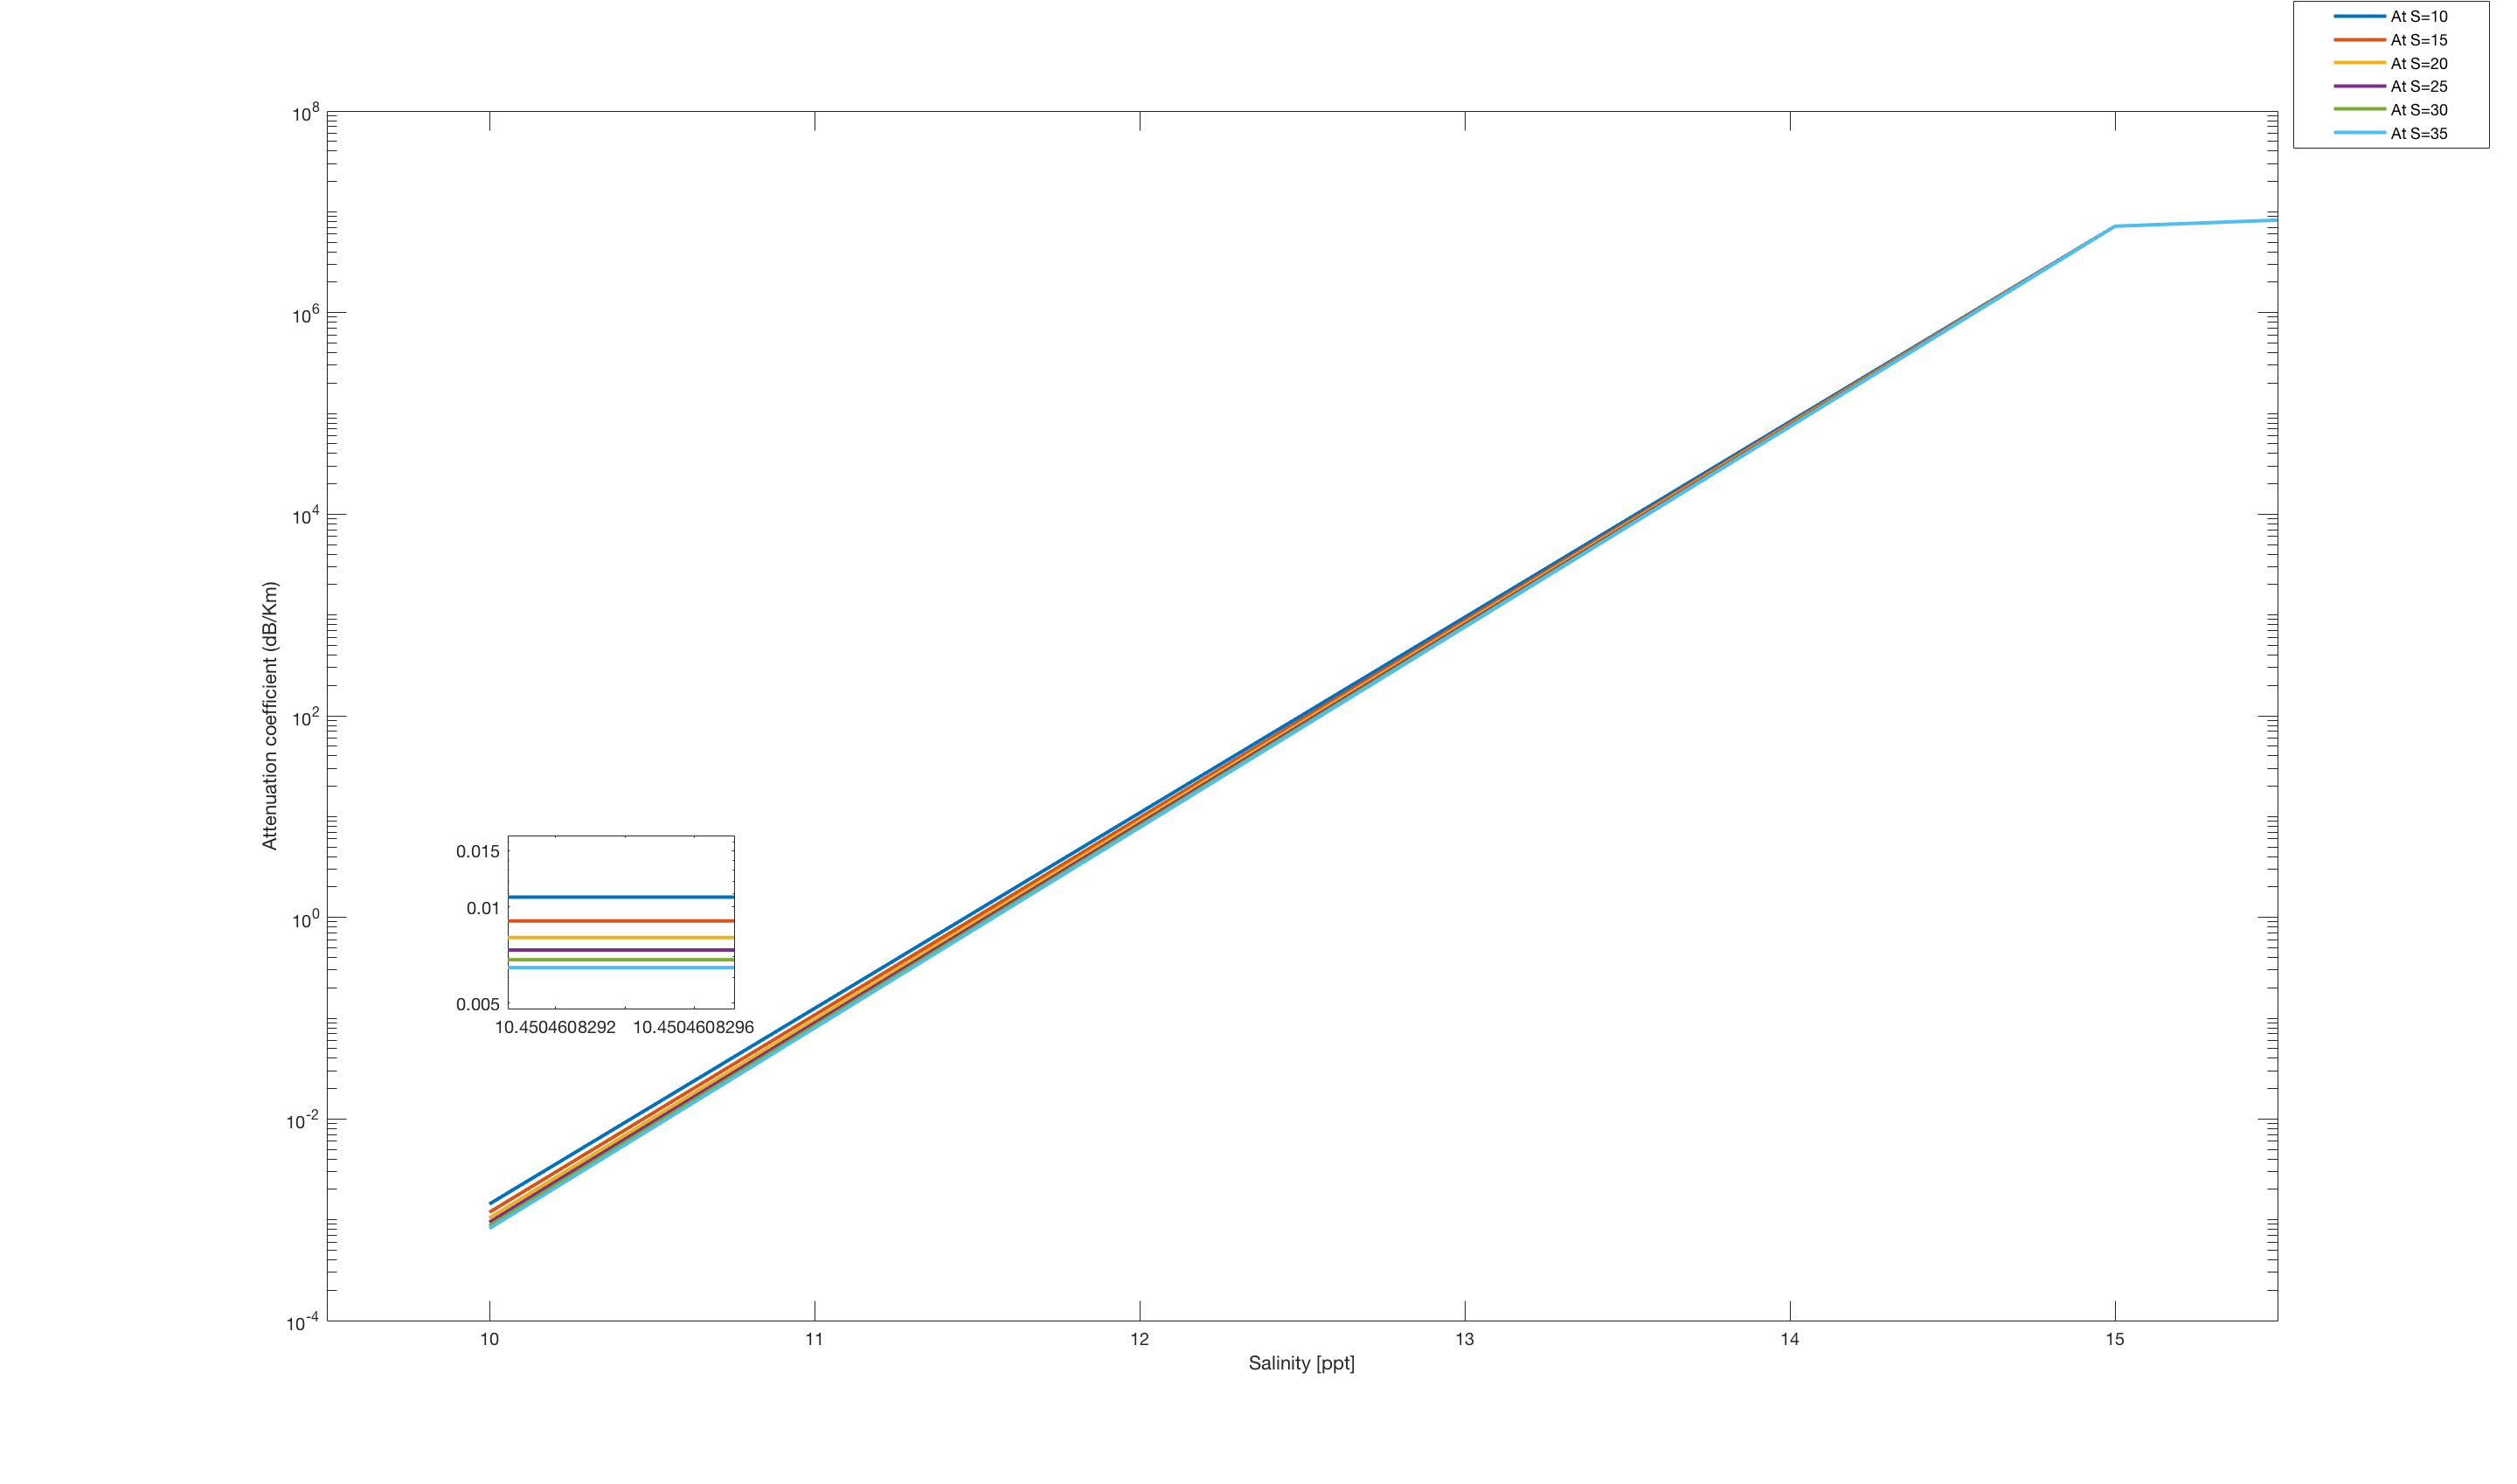
\includegraphics[scale=0.15]{ucp2_3.png}}
\caption{Dependency on salinity}
\end{figure}
\noindent A graph of salinity versus attenuation coefficient is plotted for a depth of 50m by keeping temperature and frequency constant and varying salinity. In-order to differentiate the lines for various salinities, we zoomed the graph with the help of 'magnify' function which was taken from the internet.

\subsection{Dependence on temperature} \label{Dependence on temperature} 
\noindent A graph of temperature versus attenuation coefficient is plotted for a depth of 50m by keeping salinity and frequency constant and varying temperature.
\begin{figure}[H]
\centering
{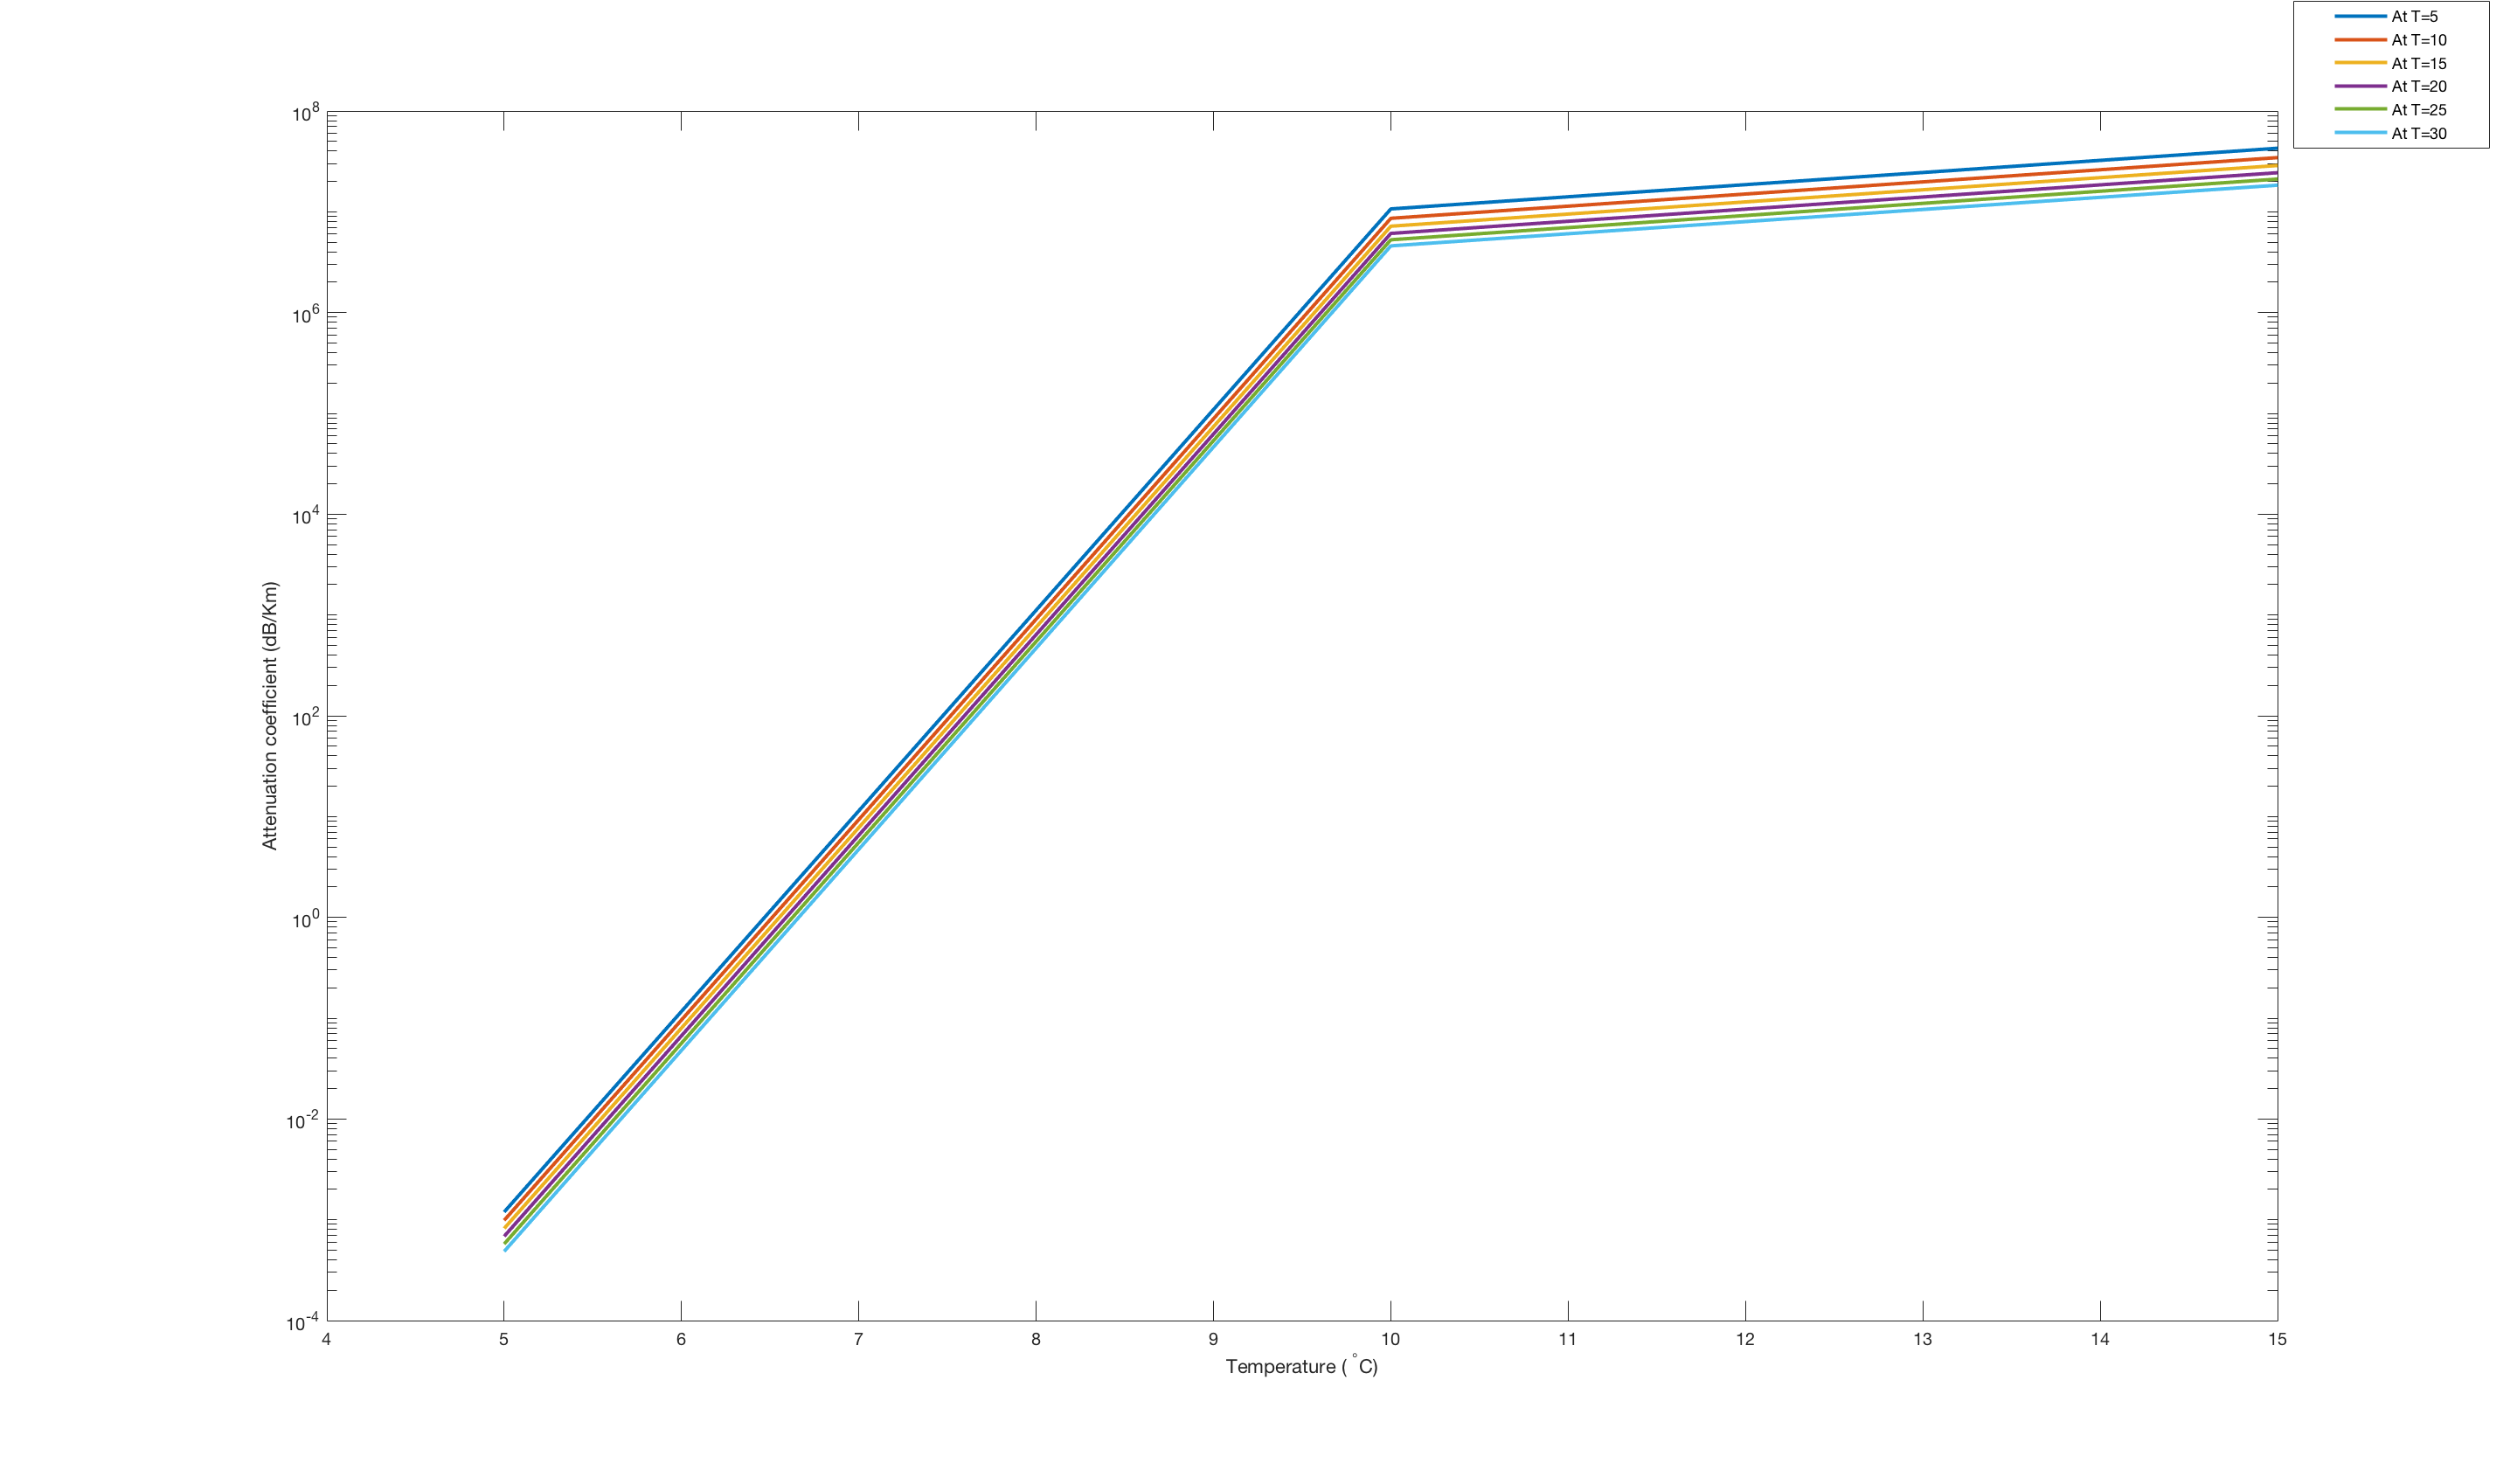
\includegraphics[scale=0.15]{ucp2_4.png}}
\caption{Dependency on temperature}
\end{figure}

\section{Attenuation versus frequency graphs for Francois and Garrison's model} \label{Attenuation versus frequency graphs for Francois and Garrison's model} 
\noindent  Set of attenuation versus frequency graphs are obtained for a depth of 50m and various values of temperature and salinity. This graph shows how temperature and salinity affect the attenuation coefficient.

\begin{figure}[H]
\centering
{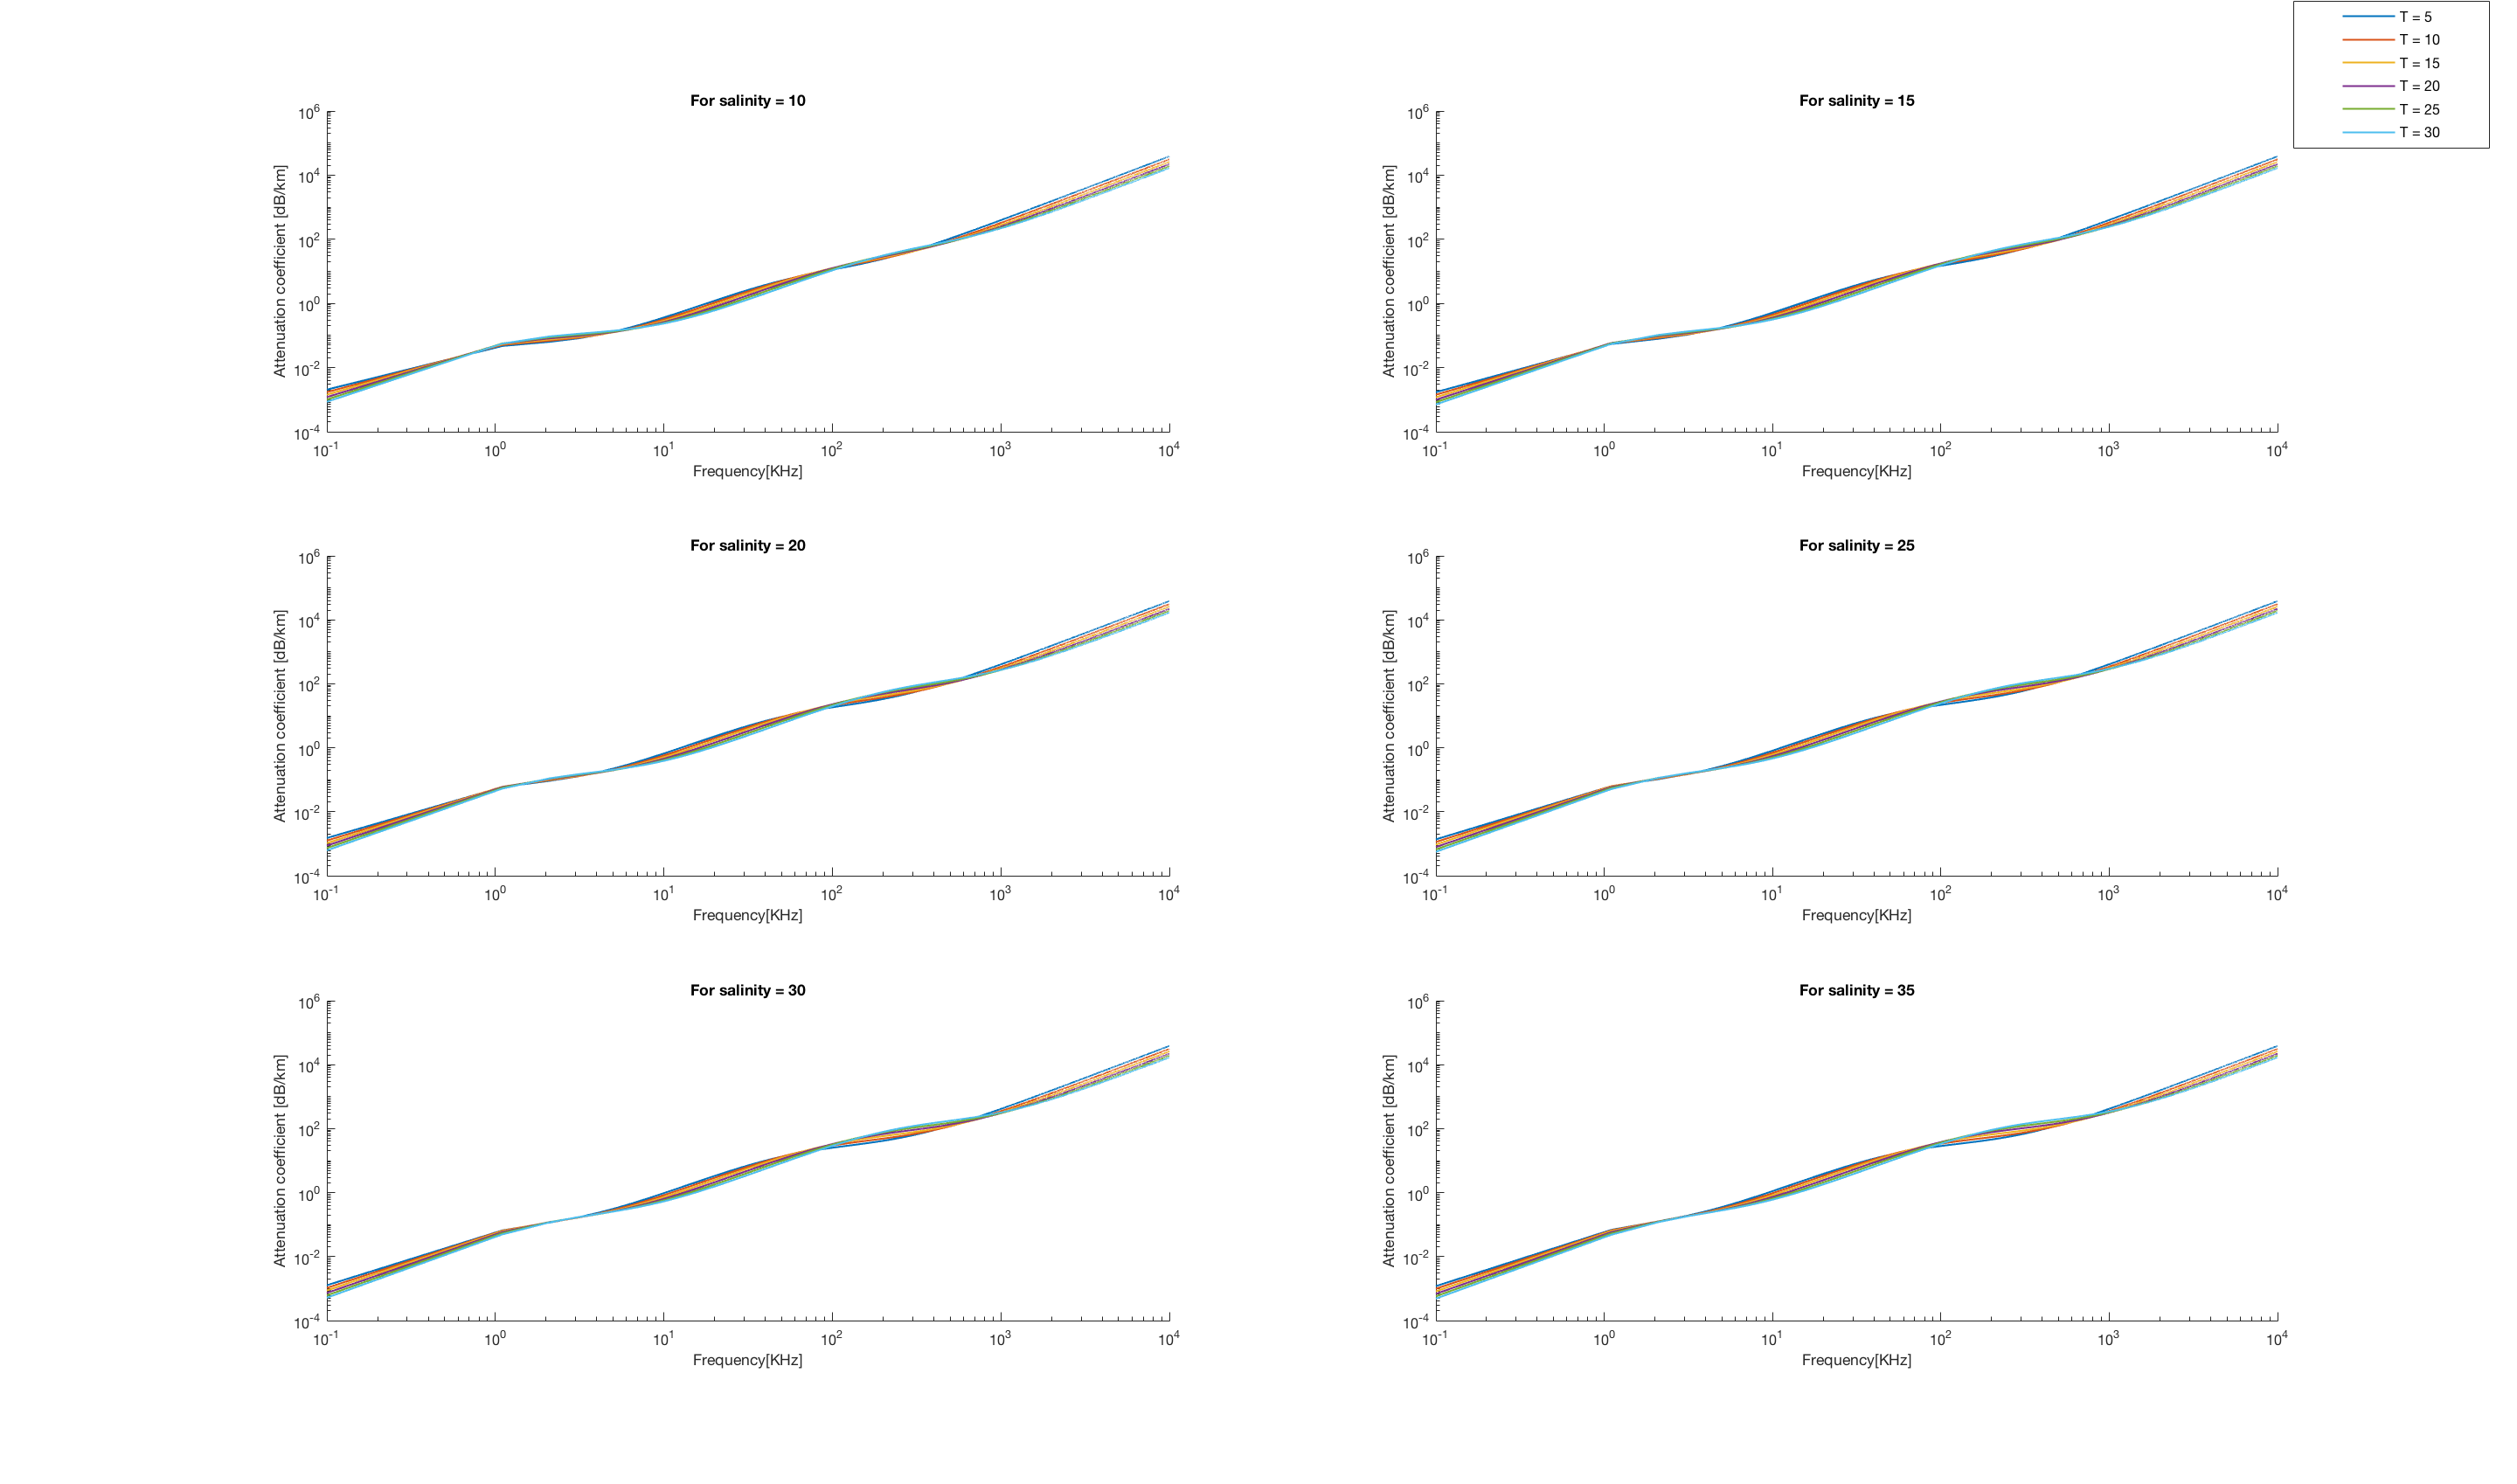
\includegraphics[scale=0.15]{ucp2_5.png}}
\caption{Attenuation versus frequency}
\end{figure}



